\documentclass{article}
\usepackage{amsmath}
\usepackage{algorithm}
\usepackage{algorithmic}
\usepackage{amssymb}
\usepackage{mathtools}
\usepackage{gensymb}
\usepackage{bbm}
\usepackage{caption}
\usepackage{subcaption}
\usepackage{graphicx}
\graphicspath{ {./pics/} }

\DeclareMathOperator*{\argmin}{argmin}
\DeclareMathOperator*{\argmax}{argmax}
\newcommand{\overbar}[1]{\mkern 1.5mu\overline{\mkern-1.5mu#1\mkern-1.5mu}\mkern 1.5mu}
\newcommand{\R}{\mathbb{R}}
\newcommand{\N}{\mathbb{N}}
\newcommand{\Z}{\mathbb{Z}}

\begin{document}

\title{Handwritten Text Recognition}
\date{September, 2019}
\author{Armand, Christopher Schuster, Mustafa Fuad Rifet Ibrahim}

\maketitle
\newpage
\tableofcontents

\newpage
\section{Introduction}
Handwritten Text Recognition (HTR) refers to the task of recognizing handwritten text from sources such as photographs, scanned documents, etc. and transcribing that to digital text (Figure 1).
Traditionally, the task of recognizing handwritten text would involve several different steps and methods such as segmenting and extracting individual characters from the lines (or pages) of scanned text and using intelligently crafted features to recognize those characters. Crafting the features is an arduous task and extracting individual characters is a challenging image recognition task in and of itself. Since 2009, when neural networks developed by J\"urgen Schmidhuber and his research group at the Swiss AI Lab IDSIA won multiple international handwritten text recognition competitions[1], neural networks became more and more prominent in the scene of handwritten text recognition. These neural networks consisted of a combination of two different architectures, namely Convolutional Neural Networks (CNN) and Recurrent Neural Networks (RNN). In this project our goal was to implement and expand a model for handwritten text recognition that uses precisely that combination of architectures. 
\begin{figure}[h]
\begin{center}
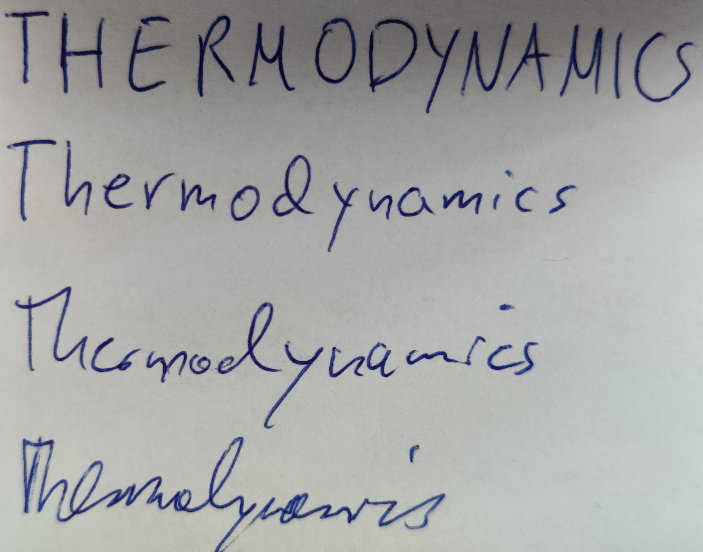
\includegraphics[scale=0.4]{text_example2}
\end{center}
\caption{Example of different levels of difficulty for handwritten text recognition. The upper example shows clear separation and writing of the individual characters while the last one shows connected and overlapping characters that are far away from their standard form.}
\end{figure}

\newpage
\section{Theory}
This section assumes basic knowledge about the concept of neural networks and the mathematics behind it. Further specific knowledge about relevant architectures will be explained.

\subsection{Convolutional Neural Networks}
Convolutional Neural Networks (CNNs) differ from the basic Fully Connected Neural Network (FCNN) in the fact that they are specifically built for processing images. In a FCNN images don't scale well, as the amount of parameters grows rapidly with increasing image size. A CNN handles this problem by having only local spatial connections between neurons of two layers. To understand how this is accomplished, two basic parts are essential, namely the convolutional layers and the pooling layers[2][3].\\\\
\textbf{Convolutional Layers}\\\\
The convolutional layer consists of filters (or kernels) that have a certain spatial extension, i.e. along the width and height of the image, and a full extension along the depth of the input. The depth of the input describes the number of channels e.g. 3 color channels in a RGB image. During the forward pass, these filters are slidden across the image and a dot product is computed between the entries of the filter and the input values of the image (Figure 2). The result is a 2D activation map (one per filter) and when these maps are stacked along the depth dimension, they represent the output volume of the convolutional layer.
The width and height dimension of the output volume are determined by three other hyperparameters: kernel/filter size, stride and padding.\\
The kernel size is the width and height of the filter window described above. The stride referrs to the amount of pixels the filter is moved along the spatial dimensions of the input at each step during the computation of the forward pass. Padding or more precisely the size of the padding refers to the size of the optional border that can be added to the input if needed. All these hyperparameters determine the width and height of the output volume according to this formula:
\[
\frac{D-F+2P}{S}+1
\]
where D is the width or height, F is the kernel size along the width or height, P is the amount of padding and S referrs to the stride length. Figure 2 also shows the concept of local connectivity mentioned above. Every entry in the output volume, or in other words every neuron, is connected to only a fraction of the input entries (or neurons).\\\\
\begin{figure}[H]
\begin{center}
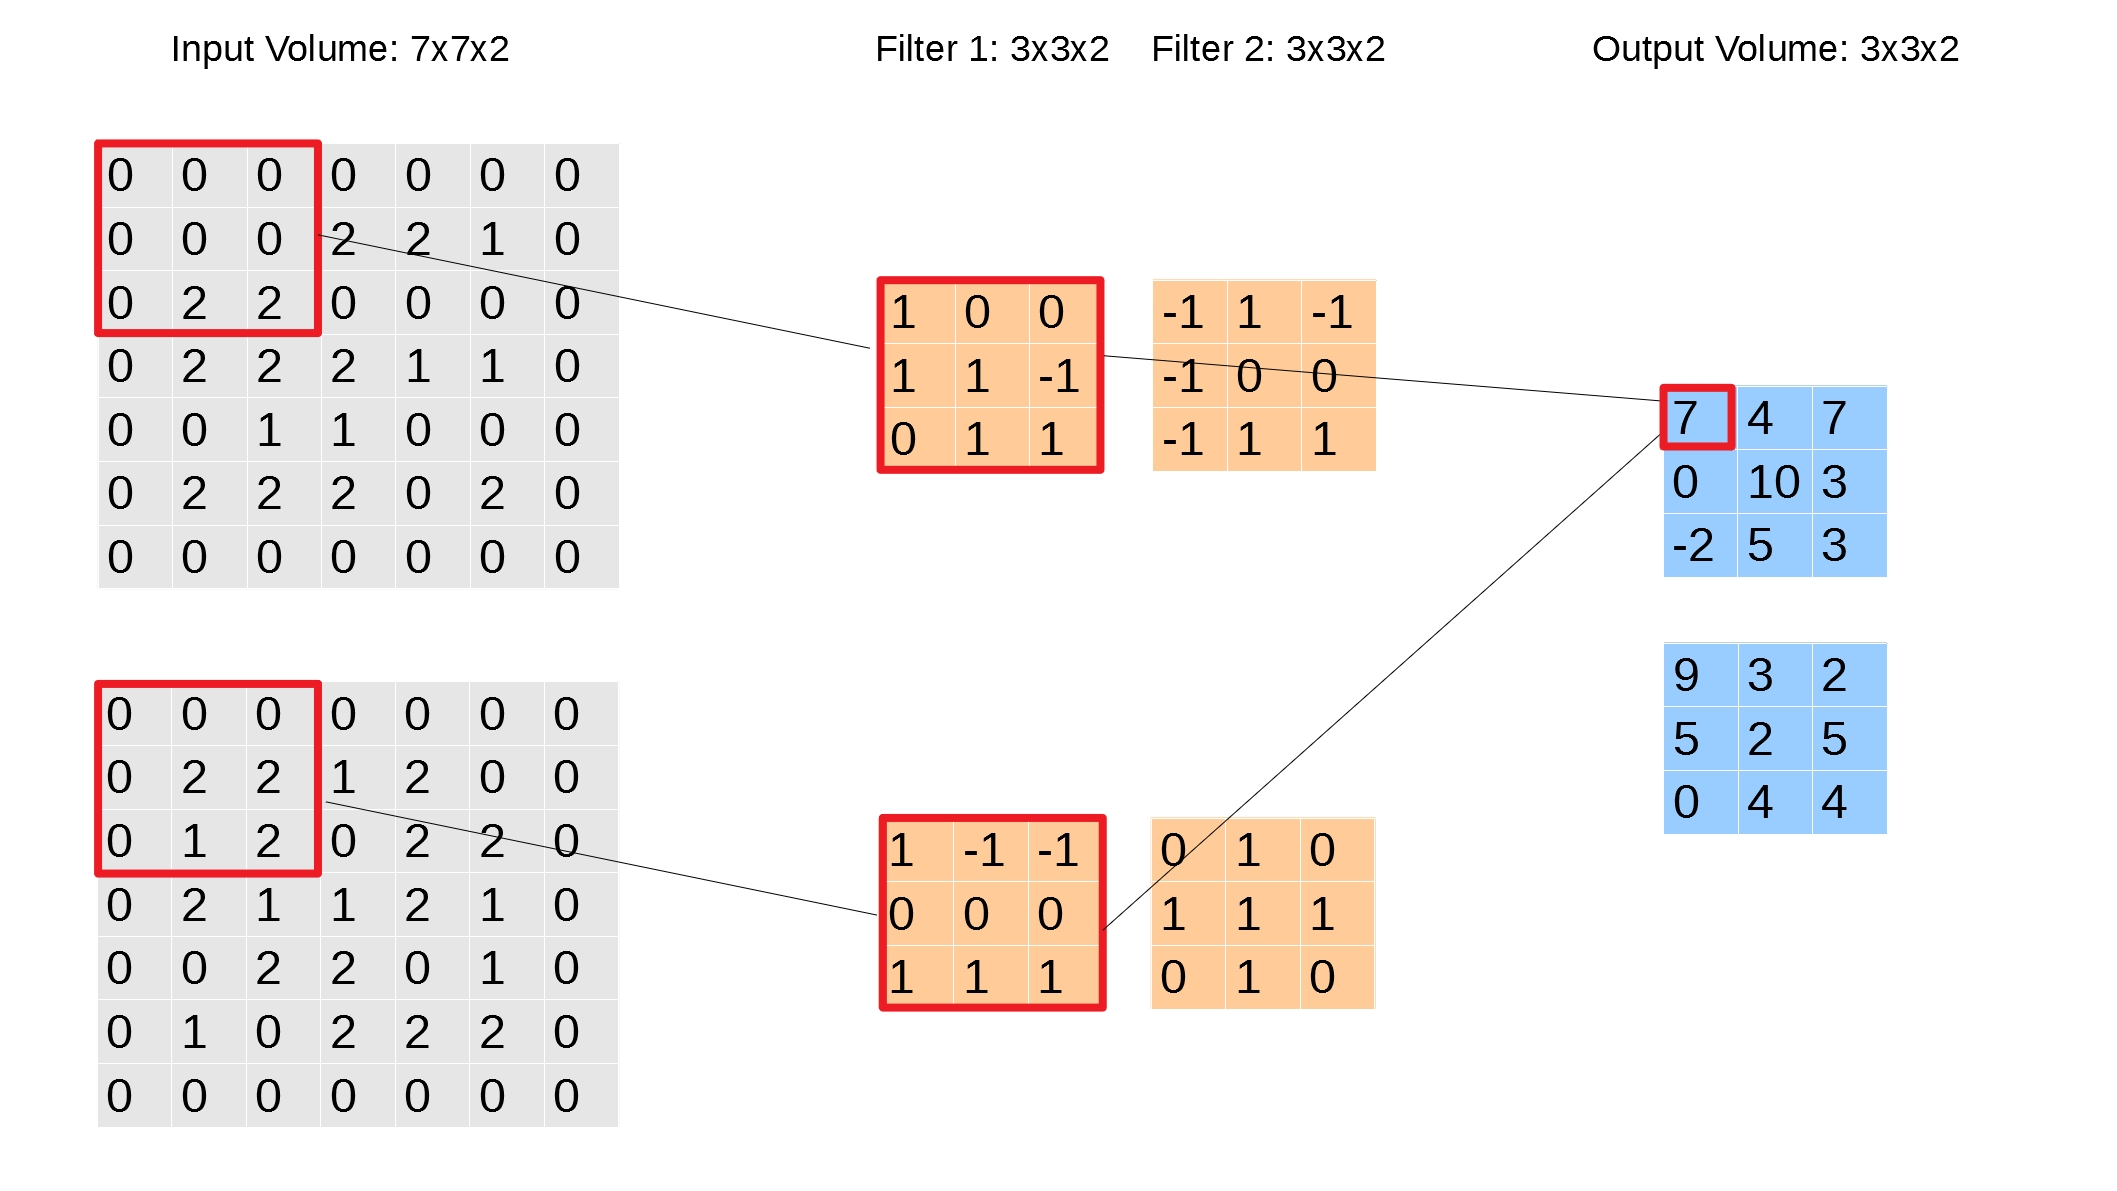
\includegraphics[scale=0.25]{CNN_forward}
\end{center}
\caption{The forward pass of the convolutional layer. On the left is the input with the size 7x7x3. It is padded with a one pixel thick border of zeros. In this graph, the depth dimension or number of channels/filters is depicted by stacking the matrices above one another. In the middle are the two filters applied to the input, in this case we have a filter size of 3x3. This gives us an output of size 3x3x2. The red squares and the black lines show the the entries of the input and the filters applied to those entries to calculate the respective output entry. }
\end{figure}
\textbf{Pooling Layers}\\\\
The pooling layers fulfill the task of downsampling the input and thus decreasing the amount of parameters (weights). The mechanics of this layer are somewhat similar to the convolutional layer. It also involves a window that is slidden across the input but in this case the max value among the input values that fall within the spatial extension of the window at the respective calculation step is taken as the output (Figure 3). This is called max pooling. There are also other functions (e.g. average function) but max pooling is the most common one. All the previously mentioned hyperparameters apply here as well except for the padding. In addition to that, the depth dimension remains unchanged as the pooling operation is done on every slice along the depth separately and the resulting downsampled slices are again stacked along the depth dimension to form the output.
\begin{figure}[H]
\begin{center}
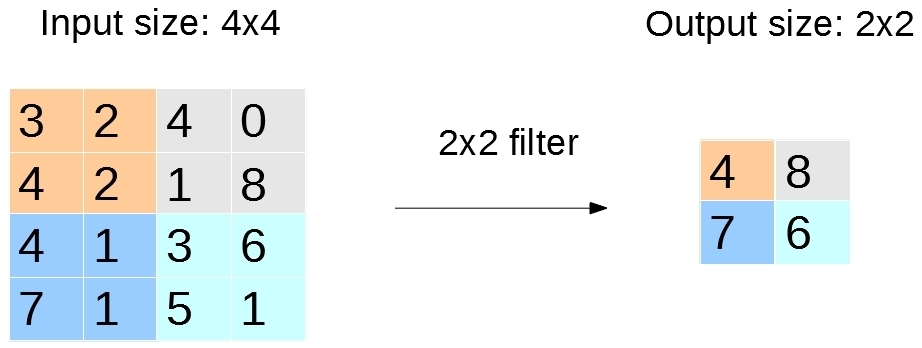
\includegraphics[scale=0.4]{rsz_1pooling}
\end{center}
\caption{The pooling operation. On the left is one depth slice of an input with width and height equal to 4. The pooling filter in this case has size 2x2 and stride 2 which effectively means that 75\text{\%} of the image information is discarded.}
\end{figure}

\subsection{Recurrent Neural Networks}
Recurrent Neural Networks (RNN) are a type of neural network architecture that allow for information of a previous inputs to persist, so that predictions can be made, within the context of the sequence of data that the features stemmed from. This enables a neural network to solve problems like guessing the most probable last word of a sentence[4].\\\\
\textbf{Vanilla RNN}\\\\
The standard RNN can be thought of as having a cell that takes in an input \(x_t\) and computes an output based on this input as well as the so called "hidden state" of the cell. This new output is then taken as the new hidden state and is combined with a new input \(x_{t+1}\) to generate the next output or hidden state. The result of the calculation can also be used to apply another function to produce an output \(y_t\) like for example some kind of class score at all time steps or only certain time steps. During all these calculation steps the same weights are used (Figure 4).
\begin{figure}[H]
    \centering
    \begin{subfigure}{1\textwidth}
        \centering
        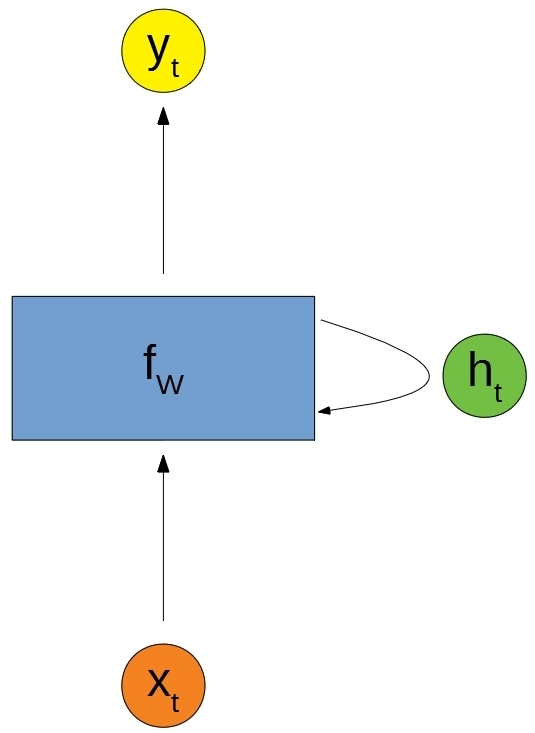
\includegraphics[scale=0.2]{rsz_rnn_roll}
        \caption{Looping visualization of RNN}
    \end{subfigure}\\
    \begin{subfigure}{1\textwidth}
        \centering
        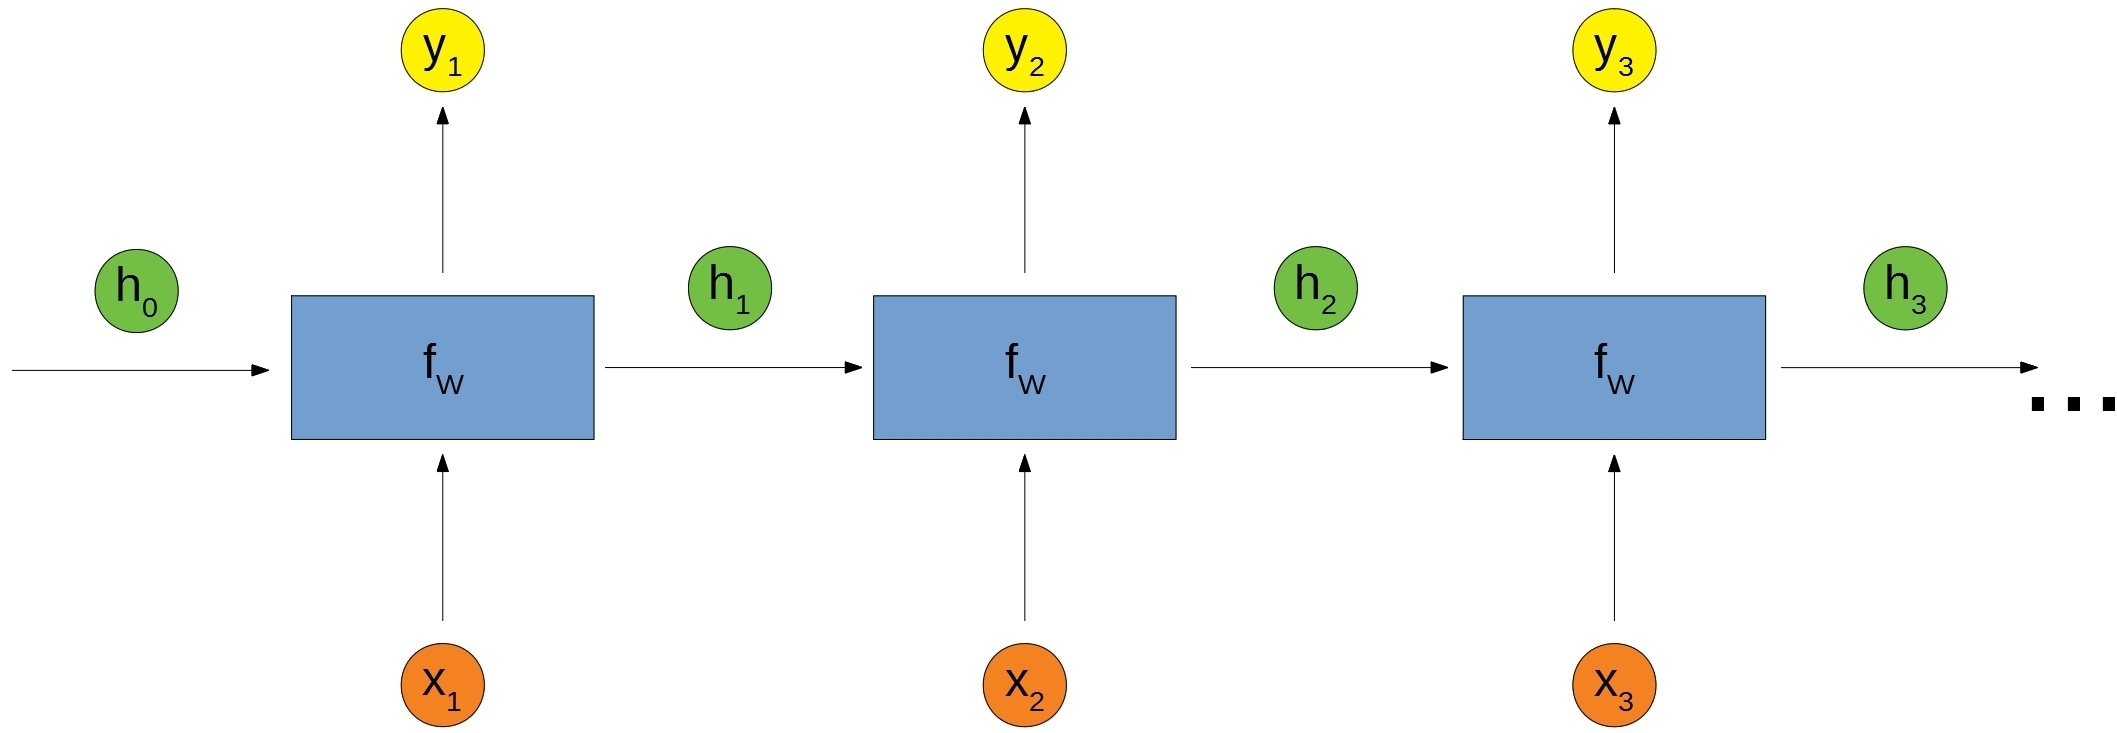
\includegraphics[scale=0.2]{rsz_rnn_unroll2}
        \caption{Unrolled visualization of RNN}
    \end{subfigure}
    \caption{Vanilla RNN visualization. f denotes the non-linear function with parameters W, h is the hidden state, x is the input and y is the output. The upper image is a visualization expressing the feedback nature of the RNN. The lower image elucidates the sequential nature of the RNN by arranging the RNN at different time steps next to itself.}
\end{figure}
The basic operation can be roughly written as:
\[
\begin{split}
h_t &= f_W(h_{t-1}, x_t)\\
y_t &= f_y(h_t)
\end{split}
\]
where the symbols have the same meaning as in Figure 4 and \(f_y\) is some function applied to get the desired output. This means that information of past sequence parts persists in the form of the hidden state. The fact that the parameters \(W\) remain unchanged for all sequence elements means that we have parameter sharing. Just like CNNs introduce a form of parameter sharing effective for image inputs, RNNs achieve the same with sequential input. This allows the RNN to not be constrained by fixed input or output size. It is also possible to increase the amount of input information by connecting two layers in opposite direction. This is called Bidirectional RNN (BRNN) and can be thought of as the combination of two RNNs, one getting the sequence input in the normal order and the other getting the input sequence in reverse order. This enables the network to produce an output based on future and past sequence information, e.g. in the case of handwritten text recognition it enables the prediction based on the letters located before and after the current letter.\\\\
\textbf{Long-Short-Term-Memory Networks}\\\\
Vanilla RNNs run into problems when it comes to long input sequences where the correctness of the output hinges on the ability to connect pieces of information that are many time steps apart. Long-Short-Term-Memory Networks (LSTM) are a RNN variant that are particularly good at handling these long term dependencies. They differ from standard RNNs in the basic module or cell that accepts the input and hidden state and produces the next hidden state or output (Figure 5). While the standard RNNs have one non-linear function in the module, LSTMs have a more complex structure that involves different functions[5].
\begin{figure}[H]
\begin{center}
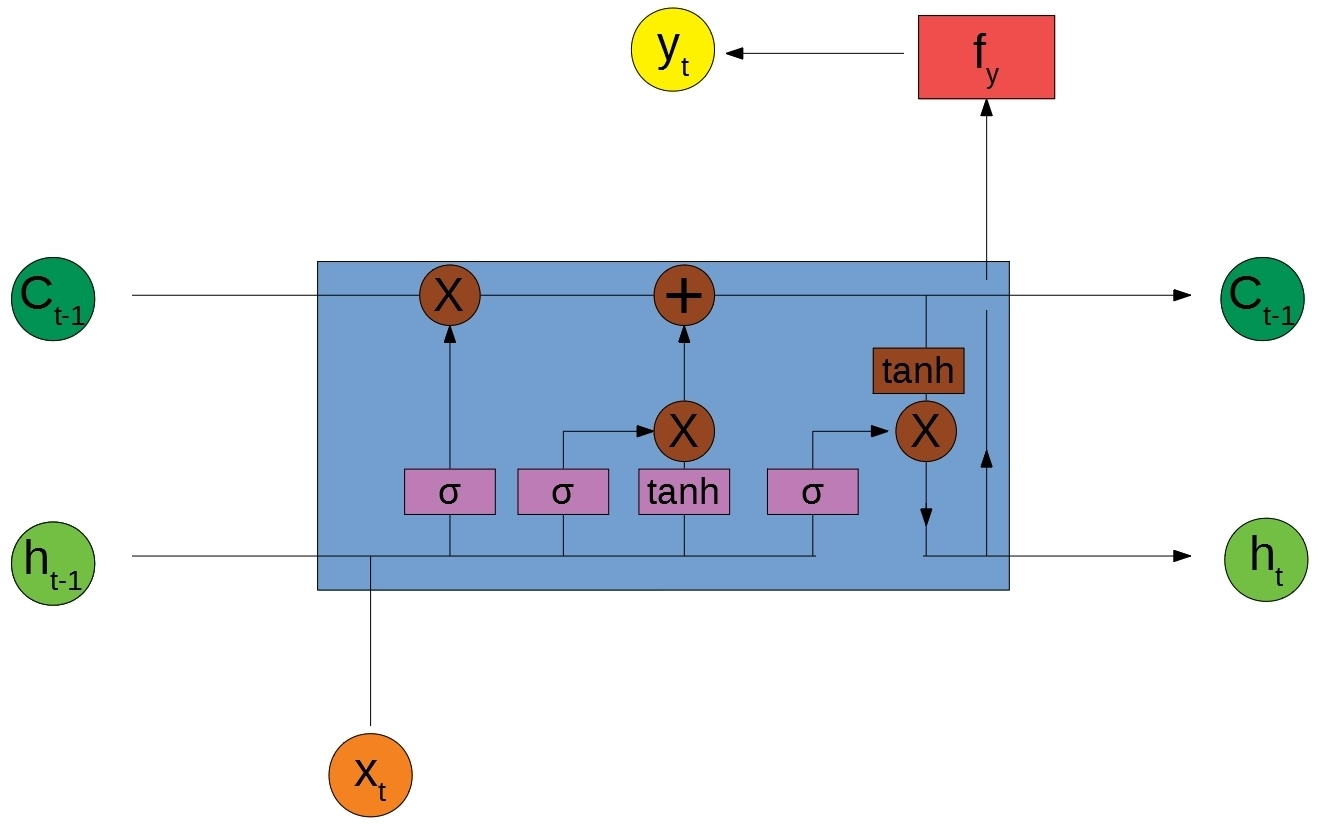
\includegraphics[scale=0.3]{rsz_1lstm}
\end{center}
\caption{LSTM Visualization. Hidden state, input and output are shown as before. The purple rectangles are neural network layers that use a sigmoid or tanh function. The brown rectangle and brown circles are point wise operations of multiplication 'X', addition '+' or a tanh function. The dark green circles are the cell state and the red square is the function used to get a desired output like for example a class score.}
\end{figure}  
As can be seen from Figure 5 the LSTM has an additional state called the cell state. This cell state flows across the upper stream and can be altered through information passing through different gates. The first one on the left is the forget gate. Here the information from the previous hidden state and the current input are used to decide which parts of the cell state to forget (values closer to 0) and which parts to keep (values closer to 1):
\[
f_t = \sigma(W_f\cdot[h_{t-1}, x_t])
\]
This gets combined with the old cell state through point wise multiplication.
Next is the input gate. Through a similar mechanism new information that is supposed to be added gets chosen here but before applying the point wise multiplication to the input, the input is pushed through a tanh layer to produce candidate values. 
\[
\begin{split}
i_t &= \sigma(W_i\cdot[h_{t-1}, x_t])\\
\tilde{C}_t &= \tanh(W_C\cdot[h_{t-1},x_t])
\end{split}
\]
This new information is combined with the old cell state through point wise addition. So to summarize the operations, the augmentation to the cell state looks like this:
\[
C_t = f_t\cdot C_{t-1}+i_t\cdot \tilde{C}_t
\]
where \(\cdot\) denotes point wise multiplication and \(+\) denotes point wise addition. The last part of the LSTM module is the output. Similar to the input gate the information is filtered. In this case the new cell state is filtered to form the new hidden state and output at that time step:
\[
\begin{split}
o_t &= \sigma(W_o[h_{t-1}, x_t])\\
h_t &= o_t\cdot\tanh(C_t)
\end{split}
\]
The tanh here is used to constrain the values of the new cell state into the range from -1 to 1 before filtering. There are many variants of this basic LSTM architecture that bring certain advantages in specfic applications but a discussion of those augmentations is beyond the scope of this report.

\subsection{Connectionist Temporal Classification}
Connectionist Temporal Classification (CTC) is the supervised learning algorithm used to train neural networks in sequential problems such as handwritten text recognition[6]. The straightforward way of doing supervised learning in this area would be to manually label every position in the input image to specify which areas of of the image are associated with which letter from the ground truth text. Then, the RNN would output its guess and the loss would punish for each character that was guessed wrong. This however is infeasible with large datasets. CTC provides a way to stop worrying about the alignment of input and output. It introduces a blank symbol that stands for no character recognized at this position to account for gaps between characters or words (or spoken words in speech recognition). It provides a way to properly decode repeat characters, and to map many different valid alignments to the ground truth.
For a given output of the RNN simply merging repeat characters and then removing any blank symbol (in that order!) provides the actual output that can be compared against the ground truth. Taking this into account, the loss is then calculated by computing the probability for all valid alignments given a ground truth text and the output of the RNN which contains the character probabilities per time step. This is done by multiplying the character probabilities for each alignment and summing over all such valid alignments. Taking the negative log of this sum gives the loss. The model parameters are tuned to minimize that loss or in other words to maximize the probability the network assigns to the right answer. To illustrate, take the following situation:
\begin{itemize}
\item ground truth text: 'bad'
\item characters: a,...,z
\item time steps(maximum word length): \(t_0\),..\(t_5\)
\item blank symbol: '-'
\end{itemize}
The following example of a RNN output matrix is given:
\begin{table}[H]
\centering
\begin{tabular}{l|l|l|l|l|l}
       & a & b & c & d &\ldots \\ \hline
\(t_0\) & 0.02 & 0.8 & 0.03 & 0.1 & \\ \hline
\(t_1\) & 0.9 & 0.01 & 0.001 & 0.03 & \\ \hline
\(t_2\) & 0.1 & 0.08 & 0.002 & 0.78 & \\ \hline
\vdots       &         &         &         & 
\end{tabular}
\caption{RNN output matrix. Only the first four letters and first three time steps are shown. The blank  symbol '-' is also part of the output and has a probability for each time step. In this case the text in the input image is likely located near the left border of the image since this example output shows high probability for the respective letters of the word appearing right at the start.}
\end{table}
With that we can calculate the probability for each valid alignment by multiplying the individual character probabilities. Valid alignments, i.e. alignments that would map to the word 'bad' if we merged repeat characters and removed blank symbols, are for example:
\begin{itemize}
\item b - - a - d
\item b b b b a d 
\item b a a a a d 
\item b a d d d d 
\item b a d - - -
\end{itemize}
If we let \(A\) be the set of all such valid alignments then the loss is calculated by taking the negative log of the sum over all the alignments probabilities:\\
\[
\text{loss} = -\log\left(\sum_A p(A)\right)
\]
\textbf{Inference}\\\\
To test the model, we need a method to extract a likely output text given the RNN output. The most intuitive way would be to simply take the alignment with the highest probability, which we call 'Best Path Decoding' in our project. This method works well if the most probable alignment has a significantly higher probability than the rest. A problem can arise when this is not the case. For example if we have only three characters: 'a', 'b' and the blank symbol '-' and we have two time steps \(t_0\) and \(t_1\), then given the following RNN output matrix:
\begin{table}[H]
\centering
\begin{tabular}{l|l|l|l}
       & a & b & - \\ \hline
\(t_0\) & 0.2 & 0.0 & 0.8 \\ \hline
\(t_1\) & 0.4 & 0.0 & 0.6 \\ \hline
\end{tabular}
\caption{RNN Output Matrix.}
\end{table}
Best Path Decoding would yield: '-' as the output because the respective alignment '- -' \(0.8\cdot 0.6 = 0.48\) has the highest probability out of all alignments. However, even though all alignments corresponding to 'a' are less probable than the one corresponding to '-', summing over them yields a higher total probability for the output text to be 'a'. 
\[
\begin{split}
\text{'a-': } 0.2\cdot 0.6 = 0.12\\
\text{'-a': } 0.8\cdot 0.4 = 0.32\\
\text{'aa': } 0.2\cdot 0.4 = 0.08\\
\text{total probability} = 0.52
\end{split}
\]
Therefore Best Path Decoding might miss some outputs that are more likely.\\
A different algorithm called Beam Search Decoding accounts for cases like these. It works by generating possible alignment candidates, expanding them by all characters and calculating the resulting probabilities of these new candidates. In each expansion step it discards all but the most probable ones, e.g. the top 10 candidates will be used in the next expansion step. So if we again have only the three characters 'a', 'b' and blank symbol '-' the first few steps of the beam search algorithm could like the tree in Figure 6.
\begin{figure}[H]
\begin{center}
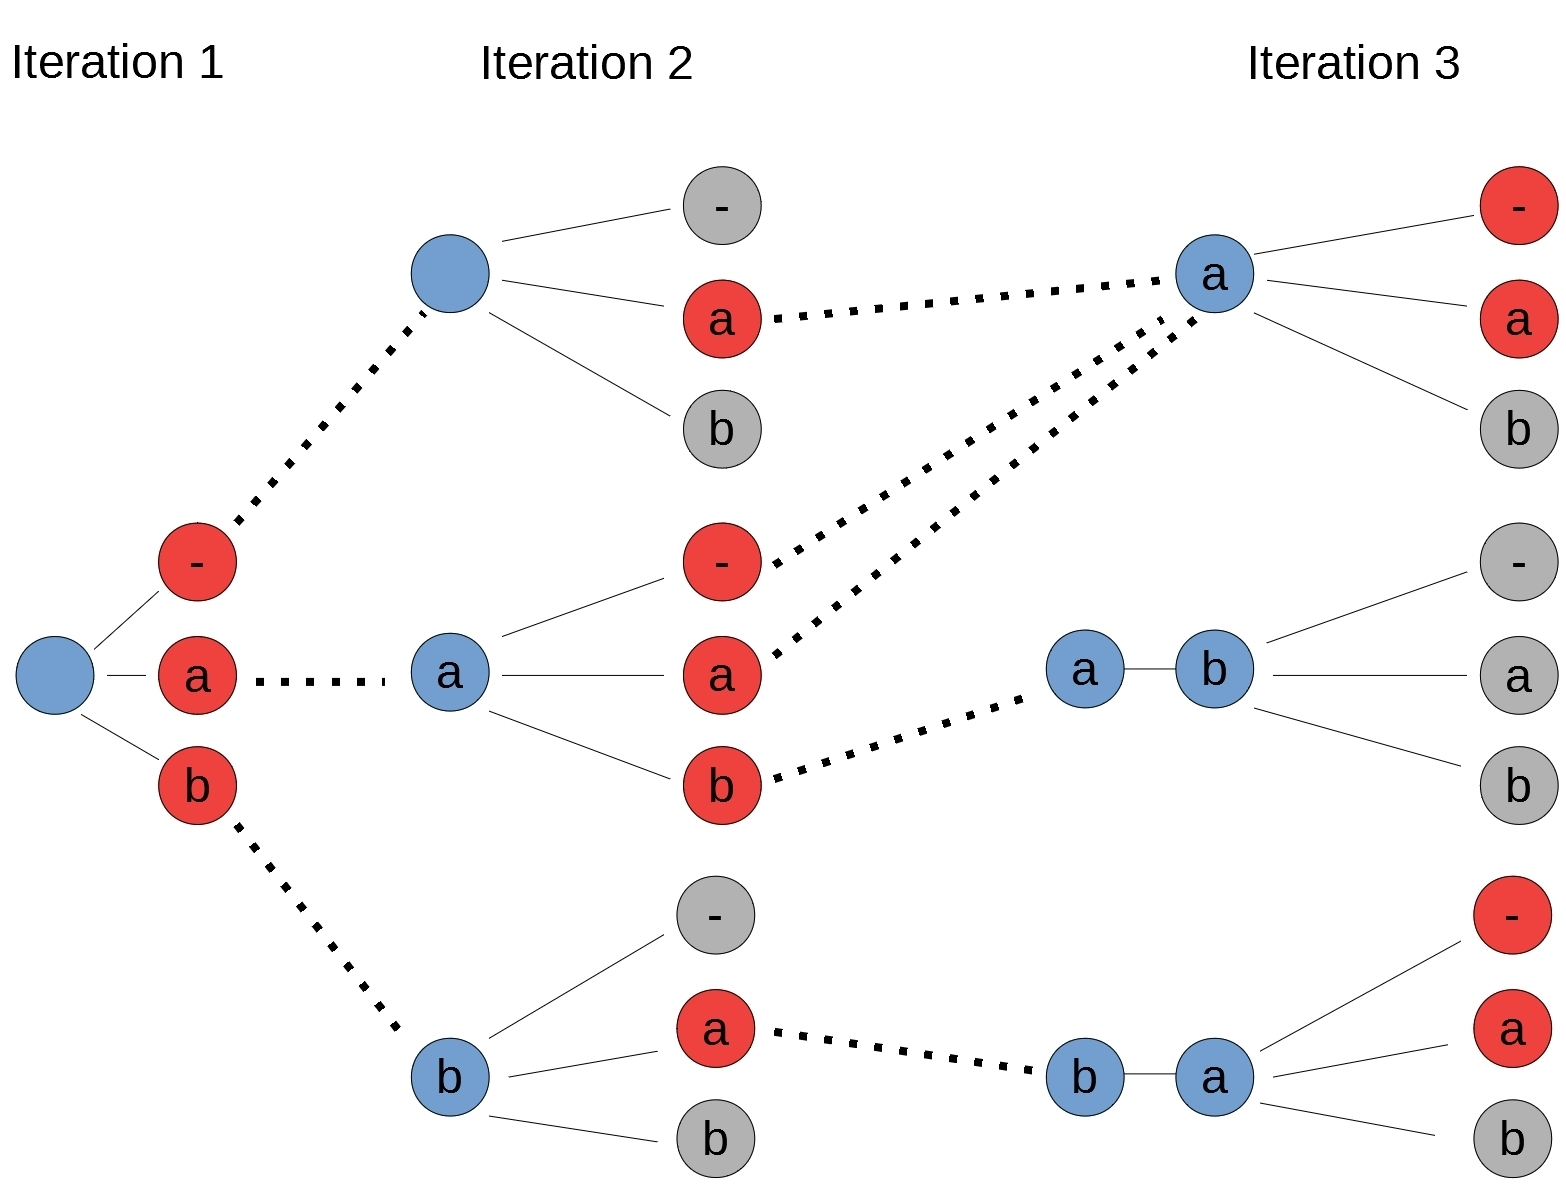
\includegraphics[scale=0.2]{rsz_beam}
\end{center}
\caption{Beam Search visualization with a tree graph. The red circles are the candidate extensions and the blue circles are the current guesses. Empty circles stand for empty strings. The dotted lines stand for the output to which the current guess plus the candidate extension map to. In each step we take the 3 most probable extended words. When multiple alignments map to one output (more than 3 circles like in Iteration 2 and 3) the probabilities are summed and summarized under one new guess. }
\end{figure}  

\newpage
\section{Methods}

\subsection{Data}
All of the input images used to train the model are from the IAM Handwriting Database[7].
In order to counteract overfitting and improve the accuracy, we applied the following transformations to the images while training: 
\begin{itemize}
\item jitter
\item translation
\item rotation
\item perspective shift
\item random erasing of pixels
\end{itemize}
For each training batch we applied these transformations with a certain probability. In addition to that we also preprocessed all images with a deslanting algorithm and tested whether or not using this deslanted training set as the default unaugmented base would result in an accuracy improvement. Figure 7 shows an example of a transformation.
\begin{figure}[H]
\begin{center}
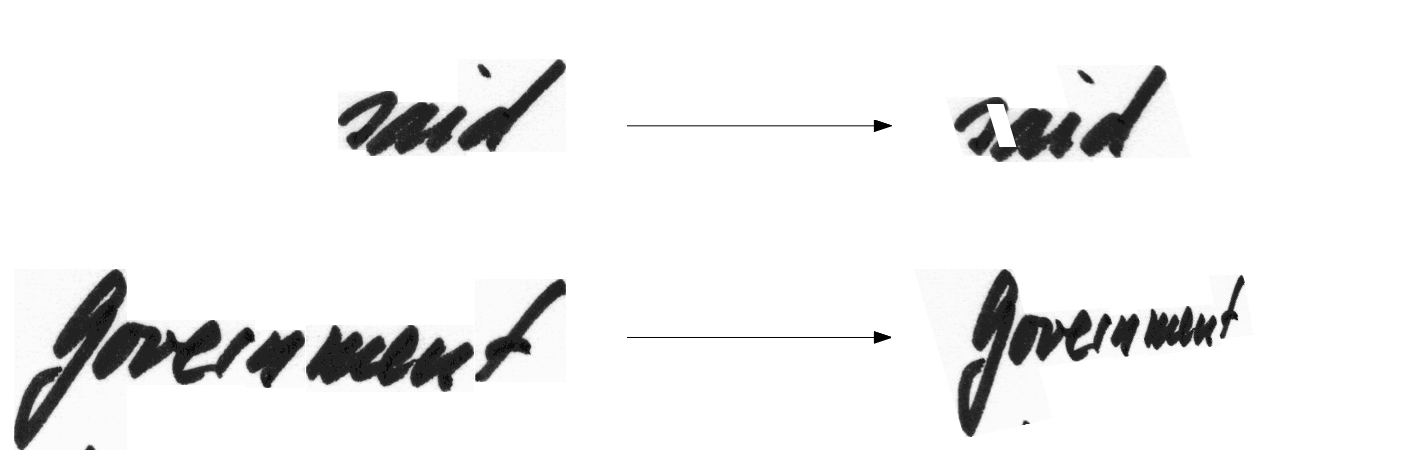
\includegraphics[scale=0.3]{rsz_transform}
\end{center}
\caption{Example of a transformation of two images. The upper image shows a random erasing of pixels and the lower image shows a perspective shift. Both images were deslanted.}
\end{figure}

\subsection{Metrics}
The main two metrics used in the field of handwritten text recognition or speech recognition are the Character Error Rate (CER) and the Word Error Rate (WER). Both of these metrics are based on measuring the Levenshtein distance between the decoded output of the model and the ground truth text. The Levenshtein distance measures the minimum amount of insertions, deletions and substitutions needed to convert one word to another, in this case output to ground truth text. CER simply normalizes this distance relative to the number of characters in the ground truth text:\\
\[
\text{CER} = \frac{\text{\#insertions}+\text{\#deletions}+\text{\#substitutions}}{length(\text{GT})}
\]\\ 
, where GT stands for the ground truth. WER works the same except for the fact that the sequence of words is used rather than the sequence of characters and that the normalization is done relative to the number of words instead of the number of characters. In addition to these metrics we also recorded the accuracy of the model as simply the percentage of correct words.
\subsection{The Model}
We based our initial approach on the Handwritten Text Recognition (HTR) system of Harald Scheidl[8][9]. Our plan was to implement that model with Pytorch as our base line performance model and test out various methods to increase the accuracy. The base model consists of two main parts, namely a Convolutional Neural Network (CNN) and a Recurrent Neural Network (RNN) with a Connectionist Temporal Classification (CTC) output (Table 3).
\begin{table}[H]
\centering
\begin{tabular}{l|l|l}
Type & Description & Output Size \\ \hline
Input & grey-scale image & 1x32x128 \\ \hline
CONV+BN+POOL & kernel 5x5, pool 2x2 & 32x16x64 \\ \hline
CONV+BN+POOL & kernel 5x5, pool 2x2 & 64x8x32 \\ \hline
CONV+BN+POOL & kernel 3x3, pool 2x1 & 128x4x32 \\ \hline
CONV+BN+POOL & kernel 3x3, pool 2x1 & 128x2x32 \\ \hline
CONV+BN+POOL & kernel 3x3, pool 2x1 & 256x1x32 \\ \hline
LSTM         & bidirectional, 2 layers, hidden size 256 & 512x32 \\ \hline
CONV         & kernel 1x1 & 80x32 \\ \hline
CTC          &      & \(\leqslant\) 32 \\ \hline
\end{tabular}
\caption{Neural Network architecture of the base line model.}
\end{table}
\textbf{CNN}\\
\begin{figure}[H]
\begin{center}
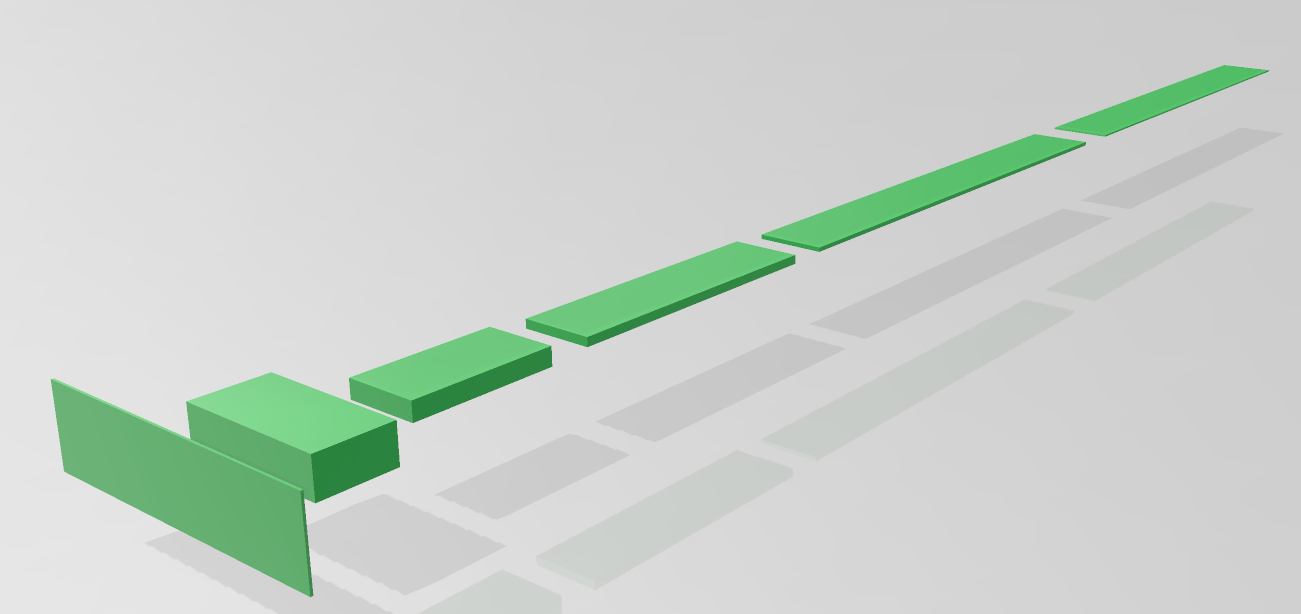
\includegraphics[scale=0.3]{CNN}
\end{center}
\caption{CNN part of the model. The first cube on the left represents the input of size 1x32x128 (channels x height x width) and the last cube on the right represents the output of size 256x1x32.}
\end{figure}
The CNN is responsible for extracting relevant features from the input images(Figure 8). All input images have the dimension 32x128 (height x width) and the CNN reduces the width to 32 and the height to 1 while extracting 256 features. In other words, the matrix at the end describes each pixel thin slice along the condensed width of the image with 256 feature values. That creates an input for the RNN that consists of 256 features and 32 time steps.\\\\
\textbf{RNN}\\
The RNN takes in the condensed sequence information and uses the extracted features in order to predict the probabilities of the possible characters in the sequence. The RNN used in this case is a Long-Term-Short-Term (LSTM) network that is bidirectional. The output of the RNN consists of a 32x256 map that contains scores for the 256 features for each time step. After the LSTM we used a single CNN layer to map the output of the LSTM to the 80 characters (english alphabet, numbers and a few additional characters plus the CTC blank symbol) that we used, resulting in a 32x80 matrix. We used the CTC algorithm to train the model, as described in the theory section, and decoded the outputs during test time with both Best Path Decoding and Beam Search Decoding. Figure 9 shows how the input matrix is transformed during the feed forward pass.
\begin{figure}[H]
\begin{center}
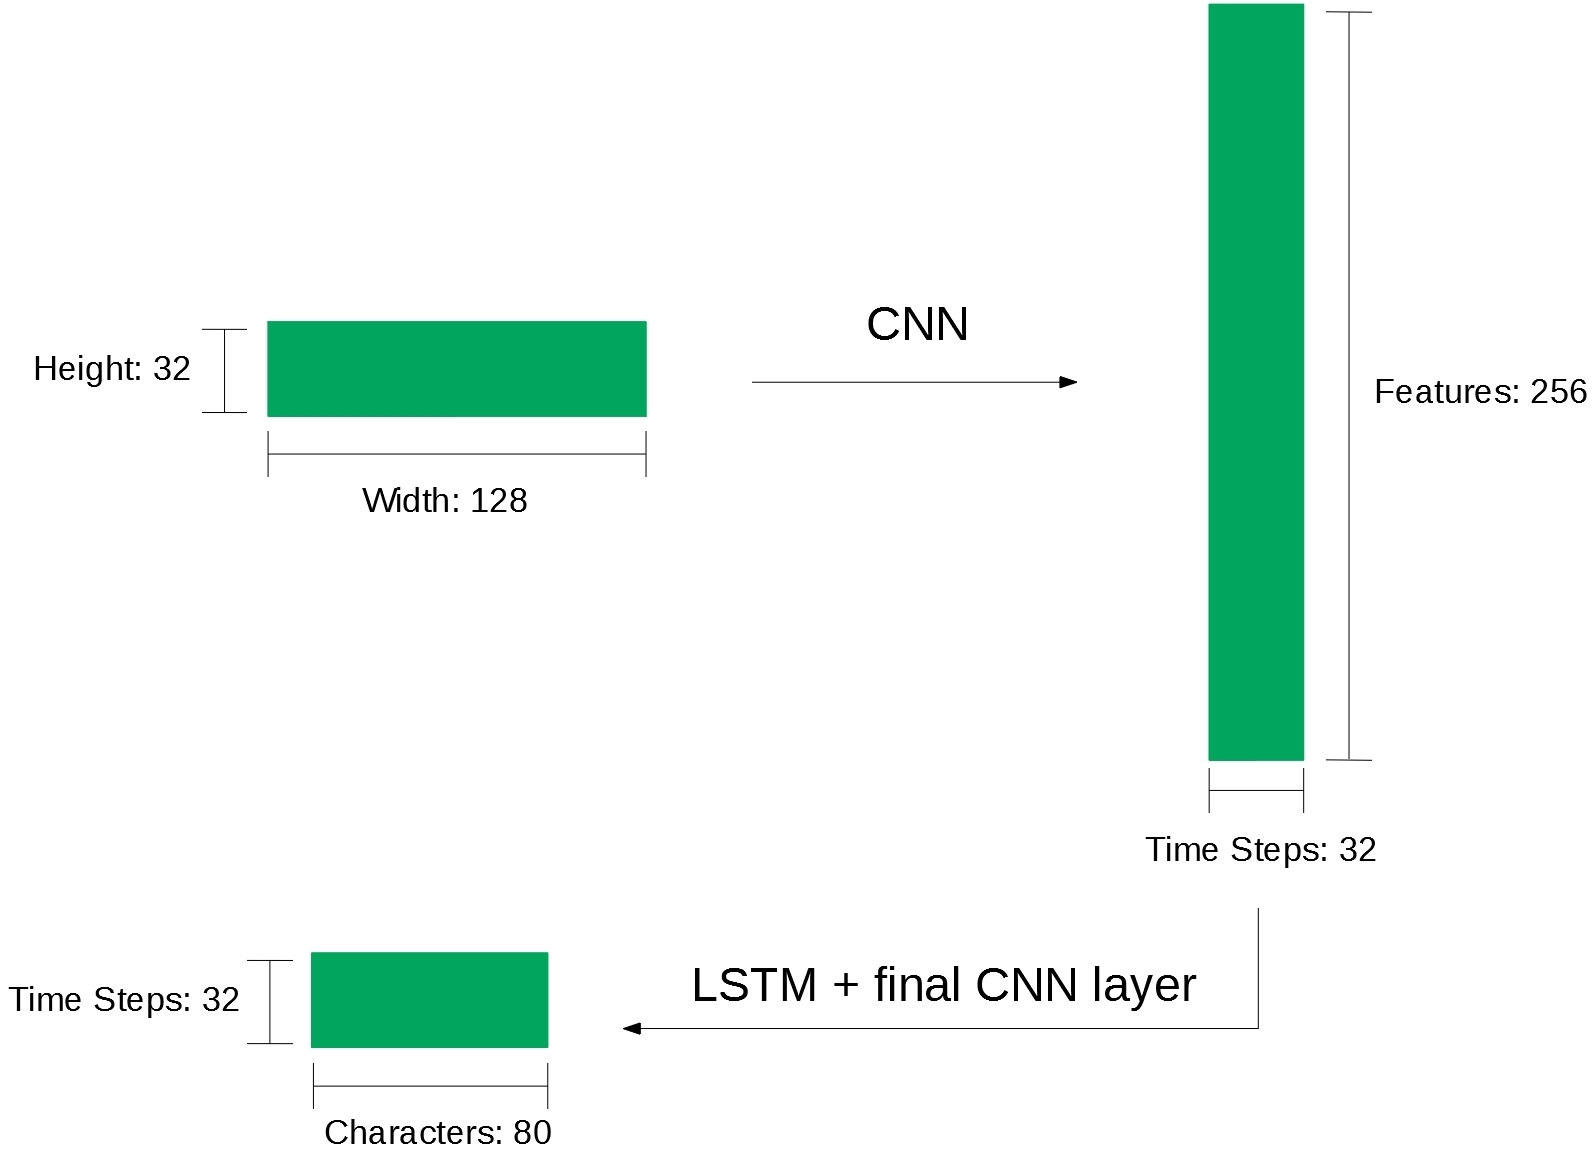
\includegraphics[scale=0.25]{rsz_pipeline}
\end{center}
\caption{Transformation through the model layers. In the top left is the input image and in the bottom left is the RNN output matrix after it was projected onto 80 characters.}
\end{figure}

\newpage
\section{Results}

\newpage
\section{Discussion}
\subsection{Text Line Recognition}
The model we built can be easily extended to recognize entire text lines, i.e. multiple words at once, by increasing the input size to make space for more words as well as adjusting the CNN layers accordingly by adding more layers and increasing the hidden size of the LSTM. An example of such a bigger model, taken from the thesis of Harald Scheidl[R], can be seen in Table 4.
\begin{table}[H]
\centering
\begin{tabular}{l|l|l}
Type & Description & Output Size \\ \hline
Input & grey-scale image & 1x64x800 \\ \hline
CONV+POOL & kernel 5x5, pool 2x2 & 64x32x400 \\ \hline
CONV+POOL & kernel 5x5, pool 1x2 & 128x16x400 \\ \hline
CONV+BN+POOL & kernel 3x3, pool 2x2 & 128x8x200 \\ \hline
CONV & kernel 3x3 & 256x8x200 \\ \hline
CONV+POOL & kernel 3x3, pool 2x2 & 256x4x100 \\ \hline
CONV+POOL+BN & kernel 3x3, pool 1x2 & 512x2x100 \\ \hline
CONV+Pool & kernel 3x3, pool 1x2 & 512x1x100 \\ \hline
LSTM         & bidirectional, 2 layers, hidden size 512 & 1024x100 \\ \hline
CONV         & kernel 1x1 & 80x100 \\ \hline
CTC          &      & \(\leqslant\) 100 \\ \hline
\end{tabular}
\caption{Example of a Neural Network architecture capable of recognizing text lines.}
\end{table}
\subsection{Deeper Network}
Deeper neural networks are commonly known to perform better since adding more non-linear layers generally leads to the ability to approximate more complex functions and be more efficient at representing certain functions[R][R][R][R]. In our case, we can deepen the network on multiple different levels.\\\\
\textbf{Deep CNN}\\\\
An obvious option is to increase the depth of the CNN of the model by increasing the number of layers.\\\\  
\textbf{Deep RNN}\\\\
Another option is to increase the depth of the RNN. There are several ways of making a RNN deeper[R].\\
The first way is to make the input-to-hidden function deeper by introducing intermediate non-linear layers. This essentially means that the temporal structure of the input sequence will be extracted based on more high level features which is advantageous because expressing relationships between more abstract features is generally speaking easier[R].\\
The second way is to make the hidden-to-output function deeper by introducing intermediate non-linear layers. This could make the prediction of the output easier which in turn would allow the hidden state to be more compact, making the model more efficient at summarizing the history of previous inputs.\\
The third way is to make the hidden-to-hidden function deeper by using a simple Multilayer Perceptron (MLP) in between. This allows the model to adapt to changing modes of the input.\\
The fourth way is to simply stack hidden layers on top of each other where the hidden states of the lower layers feed into the higher layers. This would allow the model to deal with different time scales in the input.
\subsection{Multidimensional LSTM}
The normal RNNs or LSTMs described in the theory section take in a sequence of inputs and propagate the context via one hidden state. They are inherently one dimensional and so for tasks like handwritten text recognition the input images must be reduced to only one spatial dimension, as we did using the CNN layers. Multidimensional RNNs however take in multi-dimensional inputs and use the context from those multiple dimensions in order to calculate the output[R]. This is achieved by introducing as many hidden states or recurrent connections as there are input dimensions. In our case this translates to a 2D-LSTM. Just like with standard one dimensional RNNs there is the option of choosing how to traverse the given data. In the one dimensional case the aforementioned BRNNs solve the problem by traversing the data forwards and backwards. However, if we have an image with two dimensions we can traverse the pixels in many different ways in order to gain access to surrounding contextual information. For example, one way to include context data is to traverse from the upper left corner to the lower right, meaning that the context window would be a rectangle of which the current input pixel would be the lower right corner. An example of a network utilizing this kind of LSTM, taken from the thesis of Harald Scheidl[R], can be see in Table 5.
\begin{table}[H]
\centering
\begin{tabular}{l|l|l}
Type & Description & Output Size \\ \hline
Input & grey-scale image & 1x64x800 \\ \hline
CONV+POOL & kernel 5x5, pool 2x2 & 64x32x400 \\ \hline
CONV & kernel 5x5 & 128x32x400 \\ \hline
CONV+BN+POOL & kernel 3x3, pool 2x2 & 128x16x200 \\ \hline
CONV & kernel 3x3 & 256x16x200 \\ \hline
CONV & kernel 3x3 & 256x16x200 \\ \hline
CONV+BN & kernel 3x3, pool 1x2 & 512x16x200 \\ \hline
CONV+Pool & kernel 3x3, pool 2x2 & 512x8x100 \\ \hline
MDLSTM         & bidirectional, hidden size 512 & 512x8x100 \\ \hline
Mean & average along vertical dimension & 512x1x100 \\ \hline
Dim. Reduction & remove vertical dimension & 512x100 \\ \hline
CONV         & kernel 1x1 & 80x100 \\ \hline
CTC          &      & \(\leqslant\) 100 \\ \hline
\end{tabular}
\caption{Example of a Neural Network architecture with a MDLSTM. Note that the vertical dimension was not reduced to 1 with the CNN layers, rather it was used after the LSTM to calculate an average of the output scores of the LSTM.}
\end{table}

\newpage
\section{References}
\begin{verbatim}
[1] https://www.kurzweilai.net/how-bio-inspired-deep-learning-keeps-winning-competitions
[2] Ian Goodfellow and Yoshua Bengio and Aaron Courville,
    Deep Learning pp.326-341, MIT Press, 2016
[3] http://cs231n.github.io/convolutional-networks/
[4] Ian Goodfellow and Yoshua Bengio and Aaron Courville,
    Deep Learning pp.367-390, MIT Press, 2016
[5] http://colah.github.io/posts/2015-08-Understanding-LSTMs/
[6] https://distill.pub/2017/ctc/
[7] http://www.fki.inf.unibe.ch/databases/iam-handwriting-database
[8] https://github.com/githubharald/SimpleHTR
[9] https://github.com/githubharald/CTCDecoder
[R] Bengio, Y. (2009). Learning deep architectures for AI.Found. 
    Trends Mach. Learn.,2(1), 1–127
[R] Le Roux, N. and Bengio, Y. (2010).   
    Deep belief networks are compact universal approximators.
    Neural Computation,22(8), 2192–2207
[R] Delalleau, O. and Bengio, Y. (2011). 
    Shallow vs. deep sum-product networks. InNIPS.
[R] Pascanu, R., Montufar, G., and Bengio, Y. (2013b). 
    On the number of response regions of deep feedforward networks with 
    piece-wise linear activations.arXiv:1312.6098[cs.LG]
[R] Pascanu et al, Y. (2014), 
    How to Construct Deep Recurrent Neural Networks.arXiv:1312.6026v5  [cs.NE]
[R] Mikolov, T., Chen, K., Corrado, G., and Dean, Y. (2013b).  
    Efficient estimation of word represen-tations in vector space.   
    InInternational Conference on Learning Representations:  WorkshopsTrack
[R] Graves et al, Y. (2007), Multi-Dimensional Recurrent Neural Networks.arXiv:0705.2011v1  [cs.AI]
[R] Harald Scheidl, 2018, Handwritten Text Recognition in Historical Documents,
    diploma thesis, Technischen Universität Wien
\end{verbatim}
\end{document}